%%%%%%%%%%%%%%%%%%%%%%%%%%%%%%%%%%%%%%%%%%%%%%%%%%%%%%%%%%%%%%%%%%%%%%%%%%%%%%%%%%%%%%%%%%%%%%%%%%%%%%%%%%%%%%%%%%%%%%%%%%%%%%%%%%%%%%%%%%%%%%%%%%%%%%%%%%%
% This is just an example/guide for you to refer to when submitting manuscripts to Frontiers, it is not mandatory to use Frontiers .cls files nor frontiers.tex  %
% This will only generate the Manuscript, the final article will be typeset by Frontiers after acceptance.   
%                                              %
%                                                                                                                                                         %
% When submitting your files, remember to upload this *tex file, the pdf generated with it, the *bib file (if bibliography is not within the *tex) and all the figures.
%%%%%%%%%%%%%%%%%%%%%%%%%%%%%%%%%%%%%%%%%%%%%%%%%%%%%%%%%%%%%%%%%%%%%%%%%%%%%%%%%%%%%%%%%%%%%%%%%%%%%%%%%%%%%%%%%%%%%%%%%%%%%%%%%%%%%%%%%%%%%%%%%%%%%%%%%%%

%%% Version 3.4 Generated 2018/06/15 %%%
%%% You will need to have the following packages installed: datetime, fmtcount, etoolbox, fcprefix, which are normally inlcuded in WinEdt. %%%
%%% In http://www.ctan.org/ you can find the packages and how to install them, if necessary. %%%
%%%  NB logo1.jpg is required in the path in order to correctly compile front page header %%%

\documentclass[utf8]{frontiersSCNS} % for Science, Engineering and Humanities and Social Sciences articles
%\documentclass[utf8]{frontiersHLTH} % for Health articles
%\documentclass[utf8]{frontiersFPHY} % for Physics and Applied Mathematics and Statistics articles

%\setcitestyle{square} % for Physics and Applied Mathematics and Statistics articles
\usepackage{url,hyperref,lineno,microtype,subcaption}
\usepackage[onehalfspacing]{setspace}
\usepackage{multirow}
\usepackage{pdflscape}

\linenumbers


% Leave a blank line between paragraphs instead of using \\


\def\keyFont{\fontsize{8}{11}\helveticabold }
\def\firstAuthorLast{Sample {et~al.}} %use et al only if is more than 1 author
\def\Authors{Emmanuel Devred\,$^{1}$, Tim Perry\,$^{1}$ and Philippe Massicotte\,$^{2,*}$}
% Affiliations should be keyed to the author's name with superscript numbers and be listed as follows: Laboratory, Institute, Department, Organization, City, State abbreviation (USA, Canada, Australia), and Country (without detailed address information such as city zip codes or street names).
% If one of the authors has a change of address, list the new address below the correspondence details using a superscript symbol and use the same symbol to indicate the author in the author list.
\def\Address{$^{1}$Ocean and Ecosystem Sciences Division, Bedford Institute of Oceanography,  Fisheries and Oceans Canada, Dartmouth, NS, Canada\\$^{1}$D\'epartement de Biologie, Takuvik Joint International Laboratory/UMI 3376, ULAVAL (Canada) – CNRS (France), Universit\'e Laval, Qu\'ebec, QC, Canada}
% The Corresponding Author should be marked with an asterisk
% Provide the exact contact address (this time including street name and city zip code) and email of the corresponding author
\def\corrAuthor{Emmanuel Devred}

\def\corrEmail{emmanuel.devred@dfo-mpo.gc.ca}


\begin{document}
\onecolumn
\firstpage{1}

\title[Phytoplankton absorption in the Northwest Atlantic]{Seasonal and decadal variation in phytoplankton absorption and non-algal particulate matter in the Northwest Atlantic} 

\author[\firstAuthorLast ]{\Authors} %This field will be automatically populated
\address{} %This field will be automatically populated
\correspondance{} %This field will be automatically populated

\extraAuth{}% If there are more than 1 corresponding author, comment this line and uncomment the next one.
%\extraAuth{corresponding Author2 \\ Laboratory X2, Institute X2, Department X2, Organization X2, Street X2, City X2 , State XX2 (only USA, Canada and Australia), Zip Code2, X2 Country X2, email2@uni2.edu}


\maketitle


\begin{abstract}

%%% Leave the Abstract empty if your article does not require one, please see the Summary Table for full details.
\section{}



\tiny
 \keyFont{ \section{Keywords:} Phytoplankton, absorption, chlorophyll-a concentration, phytoplankton apparent absorption wavelength ($PAAW$), Northwest Atlantic, Time series analysis} %All article types: you may provide up to 8 keywords; at least 5 are mandatory.
\end{abstract}

\section{Introduction}

I tried my best to do all requested changes. I find it difficult to keep things organized when comments are made both in mails and within the latex file.

Underwater light characteristics are important drivers of ecological processes. Among others, the magnitude of the primary productivity of photosynthetic communities \citep{Platt1980} and the photodegradation of organic matter \cite{Moran1997} are directly influenced by the quality and quantity of light penetrating the water column. The optically active constituents (OACs) controlling water’s inherent optical properties (IOPs), such as light absorption and scattering, in one ecosystem may differ fundamentally from those in another. In open water environments where the optical properties of the ocean are driven by phytoplankton, commonly referred to as case 1 waters \cite{Morel and Prieur, “Analysis of Variations in Ocean Color1.”}, absorption by phytoplankton and its detrital matter plays a key role in regulating the underwater lightscape as phytoplankton absorption alone represents more than 50\% of the total light absorption budget \citep{Oubelkheir et al., “Partitioning Total Spectral Absorption in Phytoplankton and Colored Detrital Material Contributions.”, Mascarenhas et al., “Fjord Light Regime.”}. An extensive literature has established empirical relationships between water OACs (mostly chlorophyll-a concentration and associated pigments) and their IOPs in the open oceans \citep[e.g.][]{Gordon1975, Morel1981, Kirk1981, Morel1988, Modley1994, Bricaud1995, cleveland1995,Bricaud1998, Morel2001, Ciotti2002, Bricaud2004, Devred2006, Morel2007, Brewin2011, ici il y a trop de references, aussi je ne sais pas les quelles sont manquantes et causent les ???. Peux tu me faire une liste de citation keys qui te manque? Je vais t'envoyer les liens des articles corresondants, tu pourras les ajouter à ton logiciel de gestion de références.} and polar aquatic environments \citep{Babin, “Variations in the Light Absorption Coefficients of Phytoplankton, Nonalgal Particles, and Dissolved Organic Matter in Coastal Waters around Europe.”, Matsuoka et al., “A Synthesis of Light Absorption Properties of the Arctic Ocean: Application to Semianalytical Estimates of Dissolved Organic Carbon Concentrations from Space.”,ferreira2017} \textcolor{red}{Matsuoka: https://doi.org/10.5194/bg-11-3131-2014, Ferreira:  https://doi.org/10.1002/2017JC012964}. Although that $a_\phi$ is often used as a proxy for phytoplankton biomass, it is also known to be highly influenced by the growing conditions and the physiological state of the algal assemblage and may not always truly represent the carbon content of phytoplankton cells (Behrenfeld2006).  Phytoplankton absorption coefficients, $a_\phi$ (m$^{-1}$), have also been used as indicators of phytoplankton community structure \citep{Hirata2008} and in primary production models, either directly to retrieve production \citep{, vraiment pas évident de regarder les ??? dans le pdf et de revenir à la bonne place dans le latex pour regarder si les ?? sont dues à quelles références manquantes} \textcolor{red}{10.1016/j.dsr.2006.12.001} or to weight phytoplankton light harvesting efficiency \citep{Moreal1978,kyewalyanga97} \textcolor{red}{Morel:10.1016/0146-6291(78)90623-9, Kyewalyanga: 10.1117/12.266457}. Along with $a_\phi$, the chlorophyll-specific absorption coefficient ($a^*_\phi$, absorption per unit concentration of chlorophyll-a in m$^2$ mg$^{-1}$) varies with changes in phytoplankton intracellular composition and concentration, and pigment packaging effect \citep{duysens1956,mitchell1988,kirk1975,Bricaud1995, Bricaud2004, jarrete la vérification des références ici c'est trop compliqué. Je dois regarder à chaque fois 1 par 1 voir quelle bibtext entry est manquante}\textcolor{red}{kirk1976:10.1111/j.1469-8137.1976.tb01524.x}. The exploitation of these features has led to the determination of phytoplankton size classes and taxonomic groups in natural water samples and using optical satellites \citep{Ciotti2002,Devred2006,Devred2011, Fujiki2002, Sathyendranath2004, Brewin2011}. Because phytoplankton absorption is characterized by a wide peak at around 443\,nm and a sharp maximum at around 675\,nm, empirical relationships usually focus on these two wavelengths rather than fully exploiting the spectral information contained in absorption measurements \citep{babin2003,Bricaud1995,aiken2007} \textcolor{red}{babin:  doi:10.1029/2001JC000882, Aiken: 10.1080/01431160600821036}. Still, these indices have been proven useful to study the phytoplankton dynamics in aquatic ecosystems. Absorption by non-algal particles, $a_{NAP}$ (m$^{-1}$), a ``methodological by-product'' of the determination of phytoplankton absorption derived from total particulate absorption, has been less studied than phytoplankton absorption even if its role in shaping the underwater lightscape is not negligible. Its spectral resemblance to the colored dissolved organic matter absorption spectrum has often resulted in lumping both absorptions together when solving radiative transfer issues \citep{hoge1996,maritorena2002,werdell2018} \textcolor{red}{https://opg.optica.org/ao/abstract.cfm?URI=ao-38-9-1657,  https://opg.optica.org/ao/abstract.cfm?URI=ao-41-15-2705, https://doi.org/10.1016/j.pocean.2018.01.001}. \cite{bricaud1998} \textcolor{red}{doi:10.1029/95JC00532, doi:10.1029/98JC02712.} found a significant relationship between chlorophyll-a concentration and $a_{NAP}$, however the relationship between these two variables may be location-dependent \citep{sosik1992,} \textcolor{red}{no doi for sosik92: A comparison of particulate absorption properties between high-and mid-latitude surface waters}. The ratio between total particulate absorption and $a_{NAP}$ (why use the notation for anap and not for ap?) has been found to be as low as 10\% at the surface in open oceans and reach 20\% to 30\% at depth \citep{bricaud1998}, while it can dominate the absorption budget in coastal areas \citep{babin2003,williams2018,kratzer2018} \textcolor{red}{https://doi.org/10.5670/oceanog.2018.409, https://doi.org/10.3390/rs10030418}.

Long-time series at high spatial resolution are difficult to acquire due to financial and logistical constraints. Hence, samplings in ecological studies are often carried out to study a single location over a short period such as the algal spring bloom event, or by combining data from various field campaigns that were carried out in different locations and times \citep{bricaud2004,devred2006}, which hinder our understanding of the seasonal dynamics of phytoplankton absorption. In the current study, we used an extensive and comprehensive dataset acquired within the Atlantic Zone Monitoring Program \citep[AZMP][]{casault2020} and Atlantic Offshore Zone Monitoring Program \citep[AZOMP][]{yashayaev2019} frameworks where water samples were collected over the last 20 years to describe in details the seasonal variability of chlorophyll-a concentration ([Chl-a] \,mg\,m$^{-3}$), $a_\phi$ and $a_{NAP}$ as well as their relationships in three regions of the Northwest Atlantic. We also used information on fucoxanthin pigment concentration ([Fucox]\,mg\,m$^{-3}$) as an indicator of diatom presence to help interpret the results. We also address the challenge (which one?) of using phytoplankton absorption in environmental studies to determine the status of the marine ecosystem given its complex interpretation due to its wide variation over the visible spectrum, such that the use of one or two wavelengths only truncates the information contained in an entire spectrum. We present a simple absorption index for phytoplankton (Phytoplankton Apparent Absorption Wavelength, $PAAW$) that was inspired by the work of \citep{Vermeulen2020} who applied this concept to remote sensing reflectance. This index summarizes all the spectral information contained in measured phytoplankton absorption spectra into a single number (nm) that provides information on the biomass and structure of the phytoplankton community without the need for chlorophyll-a concentration. Our large datasets provided us with the ability to detect possible changes in $PAAW$ at the regional scales over two decades and to test the minimum sampling requirement to capture the natural variability of the Northwest Atlantic ecosystem. 

\section{Material and Methods}

\subsection{Study area and sampling}

Since 1999, the Department of Fisheries and Oceans Canada (DFO) conducts annual surveys in the Northwest Atlantic as part of the Atlantic Zone and Atlantic Offshore Zone monitoring programs \cite{therriault1998,Pepin2005} \textcolor{red}{no dio for Theriault: THERRIAULT, J.-C., B. PETRIE, P. PEPIN, J. GAGNON, D., GREGORY, J. HELBIG, A. HERMAN, D. LEFAIVRE, M., MITCHELL, B. PELCHAT, J. RUNGE, and D. SAMEOTO., 1998. Proposal for a Northwest Atlantic Zonal Monitoring Program. Canadian Technical Report of Hydrography and Ocean, Sciences 194: vii + 57 pp}. On perd vraiment le flow de lecture quand on arrive à un endroit comme ici avec du code latex. Each year, in spring sometimes between April and June, depending on ship availability and weather, about 100 stations are sampled on the Scotian Shelf/Gulf of Maine region and 28 stations are sampled in the Labrador Sea along a transect that spans from the Labrador Shelf (Canada) to the Greenland Shelf (Denmark), crossing the Labrador Basin (Figure \ref{fig:1}). The spring cruise on the Scotian Shelf is repeated in the fall from mid-October to mid-November. Fish surveys that happened during winter and summer opportunistically provided additional water samples. For this study, a total of 3279 sampling events were compiled and grouped into three bioregions, namely the Scotian Shelf, a temperate mesotrophic environment, the Northwest Atlantic Basin, and a temperate oligotrophic environment and the Labrador Sea, a sub-arctic environment. The delineation of these bioregions was based on bathymetry (GEBCO2021) and the latitude (Supplementary Figure S1): (1) Scotian Shelf (bathymetry $<$ 600\,m and latitude $<$ 48$^\circ$N), (2) Northwest Atlantic Basin (bathymetry $\ge$ 600\,m and latitude $< 48^\circ$N) and (3) Labrador Sea (latitude $\geq 48^\circ$N). Observations were further grouped into seasons based on the time of sampling (Supplementary Figure S1B): spring (Mar, Apr, May, $N$ = 1598), summer (Jun, Jul, Aug, $N$ = 369), autumn (Sept, Oct, Nov, $N$ = 1174) and winter (Dec, Jan, Feb, $N$ = 138). At each station, surface water ($<$ 30\,m) was collected to measure phytoplankton pigment composition and particulate absorption.

\subsection{Data and laboratory analysis}

\subsubsection{Chlorophyll-a and Fucoxanthin pigment concentration}

Samples for pigment analysis were filtered at low pressure ($<$ 10\,dpi) on 25\,mm WF/F Whatman filters (sterlitech Grade F Glass microfiber) with 0.2\,$\mu$m mesh size and immediately flash frozen and stored in Nitrogen Liquid during the sea-going fieldwork. The volume of filtration varied between 0.25 and 1\,L based on a visual inspection of the filter colour to ensure that enough material was retained for analysis. Upon return to the Bedford Institute of Oceanography, the samples were stored inside a -80$^\circ$\,C freezer until analysis in the laboratory. Pigments composition and concentration were measured on a Beckman–Coulter Gold High-Performance Liquid Chromatography (HPLC) system between 1998 and 2013, and on an Agilent 12000 HPLC system for data collected between 2013 and 2020. Details on the HPLC method to extract and measure pigment concentration can be found in \cite{Head1993}. In this study, we limited the pigment to chlorophyll-a and derivative ([Chl-a] in mg m$^{-3}$) and fucoxanthin ([Fucox] in mg m$^{-3}$) concentration, the latter being used as a coarse indicator of diatom presence in samples.

\subsubsection{Absorption coefficient of phytoplankton and non-algal particulate matter}

Filtration for phytoplankton ($a_\phi$) and non-algal particles ($a_{NAP}$) absorption coefficients were carried out simultaneously as filtration for pigment analysis following the same protocol (i.e., filtration and storage method). Phytoplankton absorption coefficients between 350 and 750\,nm were measured at 1\,nm increment on a UV-Vis Shimadzu 2600i double beam with an integrating sphere in transmission mode. Only the visible part of the spectrum (400-700\,nm) was used in the current study. Total particulate absorption coefficient ($a_p$) was measured first, after which, the filter was soaked in hot methanol for 25 to 45 minutes to extract phytoplankton pigments. The absorption by non-algal particles, also referred to as detritus absorption, was then measured, and phytoplankton absorption was inferred by subtraction of $a_{NAP}$ to $a_p$ as described in \cite{mitchell1984} \textcolor{red}{$https://doi.org/10.1007/978-3-662-02401-0_135$} following modifications by \cite{Hoepffner1991}\textcolor{red}{http://www.jstor.org/stable/24825388} and \cite{Kyewalyanga1997} \textcolor{red}{10.3354/meps146207}. The pathlength correction (i.e., the $\beta$-factor) was computed as in \cite{Stramski2015}\textcolor{red}{ https://doi.org/10.1364/AO.54.006763}. Two quality control procedures were used to ensure the integrity of the absorption dataset; spectra were removed from further analysis if: (1) negative values occurred between 350 and 400\,nm and (2) the absorption coefficient at 410\,nm was higher than the one at 443\,nm as in \cite{devred2006}. The slope of the exponential decrease of the particulate absorption spectrum, $S_{NAP}$ was computed by fitting the following equation to the data using the \textit{nls()} function in R over the range 400 to 700\,nm excluding the 400 to 480 and 620 to 700\,nm ranges to avoid possible contamination by pigment remaining from the extraction:
\begin{equation}
a_{NAP}(\lambda) = a_{NAP}(443) (-S_{NAP} (\lambda - 443)).
\end{equation}

\subsection{Statistical Analysis}

\subsubsection{Phytoplankton apparent absorption wavelength}\label{paaw}

To summarize the spectral information contained in phytoplankton absorption measurements in a simple index, we used a method similar to that of \cite{Vandermeulen2020}. The formulation of this index was initially proposed to maximize the utilization of the spectral information contained in remote sensing reflectance, and simply represents the weighted harmonic mean of a spectrum. As pointed out by \cite{Vandermeulen2020}, but adapted to our study (what was adapted exactly?), the index indicates the wavelength balance point around which absorption is evenly distributed. Since we are adopting this index to characterize the spectral shape of in situ phytoplankton absorption, we named this index the phytoplankton apparent absorption wavelength ($PAAW$, nm), which was calculated as follows:
\begin{equation}
PAAW = \frac{ \sum\limits_{\lambda = 400}^{\lambda=700} a_\phi(\lambda)} {\sum\limits_{\lambda = 400}^{\lambda=700} a_\phi(\lambda) /  \lambda}% \frac{a_\phi(\lambda)}{\lambda}
\end{equation}
Where $a_\phi(\lambda)$  is the measured phytoplankton absorption measured at the wavelength $\lambda$ (nm).

\subsubsection{Regression and trend analysis}
The relationship between phytoplankton absorption coefficient at a given wavelength and [Chl-a] was derived using a type-2 linear regression on the log10-transformed data (when required to achieve normality). Times series analysis of the $PAAW$ was performed on data collected in spring and autumn only (except for the Labrador Sea in autumn), as there were no sufficient years with data in winter and summer to obtain reliable trends. For all-time series, namely the entire dataset, the three datasets partitioned into regions and the five datasets partitioned into seasons and regions, the mean $PAAW$ was computed and its trend was derived using a weighted general linearized model ($glm()$ in R). The weights for the fit were derived using the number of data available in any given year/region/season and the model included the latitude and longitude to account for any possible geographical bias in the linear regression due to sampling. The coefficient derived for the annual independent variable was used to describe the trend. 

All data manipulation and statistical analysis were performed in R 4.1.2 (refs) and all the data used in this study are available on Zenodo (add link). The R packages used in the study include: \textcolor{red}{include list here}

All these extra analyses with lon lat, glm etc. that were requested, are not used?

\section{Results}

\subsection{[Chl-a], [Fucox], absorption coefficients and $PAAW$ seasonal and regional variations}

For the three biogeochemical regions, both mean [Chl-a] and [Fucox] were highest in spring when phytoplankton bloom and the community assemblage is dominated by diatoms with values of 2.70, 1.80 and 2.73\,mg\,m$^{-3}$ for [Chl-a] on the Scotian Shelf, NAB and the Labrador Sea, respectively,  and values of 0.89, 0.47 and 0.72\,mg\,m$^{-3}$ for [Fucox] on the Scotian Shelf, NAB and the Labrador Sea, respectively (Table \ref{tab:1}). The Scotian  Shelf showed the highest seasonal variability with a strong decrease of both [Chl-a] and [Fucox] in summer followed by an increase during fall and a second decrease in winter for [Chl-a] that remained higher than the mean summer values, while [Fucox] in winter was greater than in Fall (Figure \ref{fig:2}). Both [Chl-a] and [Fucox] in NAB followed the same seasonal pattern as on the Scotian Shelf, but with smaller mean values. The Labrador Sea exhibited a  different seasonal cycles than the two other regions, as both [Chl-a] and [Fucox] continuously decreased during summer, fall and winter to reach the lowest values of all regions and seasons (i.e., [Chl-a] = 0.19\,mg\,m$^{-3}$ and [Fucox] = 0.05\,mg\,m$^{-3}$). The similar seasonal cycle between [Chl-a] and [Fucox] is supported by the high degree of correlation between the two pigments (0.85, Figure \ref{fig:3})


Measured absorption coefficients at 443\,nm for particulate, non-algal and phytoplankton spanned about three orders of magnitude and followed a normal distribution when log\textsubscript{10}-transformed (Figure \ref{fig:S2}). All properties showed large regional and seasonal variabilities (Table \ref{tab:1} and figure \ref{fig:3}, fig3 is showing only 2 parameters). Data revealed the same seasonal cycle for $a_\phi(443)$ than for [Chl-a] with the exception that $a_\phi(443)$ was slightly higher in the fall (0.059\,m$^{-1}$) than in the spring (0.050\,m$^{-1}$) on the Scotian Shelf (Fig. xxx). The absorption coefficient at 675\,nm (Fig. 2B, we have so (too) many figures in the paper, have to hold the hand of the reader and point out every figure/panel to support the text) exhibited the same seasonal cycle as $a_\phi(443)$ with smaller values as expected. The specific absorption coefficient at 443\,nm showed an inversed pattern to [Chl-a] and $a_\phi(443)$ in all regions, perhaps with less variability between summer and fall on the Scotian Shelf compare to $a_\phi(443)$ and the notable exception of the low mean  $a^*_\phi(443)$ in the Labrador Sea when [Chl-a] is also low. Absorptions coefficient at 443\,nm by non-algal particulate matter exhibited a different seasonal pattern than $a_\phi(443)$ on the Scotian Shelf, with high values reached in the spring followed by a decrease in Summer and an increase for both fall and winter. In the NAB, $a_{NAP}(443)$ was highest in spring, with values relatively low (0.0051\,m$^{-1}$) compared to the Scotian Shelf (0.009\,m$^{-1}$) and Labrador Sea (0.0075\,m$^{-1}$).  For the rest of the year,  $a_{NAP}(443)$ remained quasi constant with values of about 0.0035\,m$^{-1}$ (ANOVA test p-value < 0.05). In the Labrador Sea, $a_{NAP}(443)$ showed a similar seasonal pattern to $a_{\phi}(443)$ with a continuous decrease from spring to winter, unlike the two other regions where markedly different seasonal patterns were observed. The slope of the $NAP$ absorption spectrum also shows very weak seasonal dependence, with a slight decrease from spring to winter on both the Scotian Shelf and NAB, while $S_{NAP}$ reaches a minimum in fall in the Labrador Sea. 

The $PAAW$ provided additional information than [Chl-a], $a_\phi(443)$ and $a^*_\phi(443)$. On the Scotian Shelf, $PAAW$ exhibited a seasonal cycle that resembled the one of $a^*_\phi(443)$ with a mean value of  483\,nm in Spring that decreased to 470\,nm in Summer to increase again in autumn (478\,nm) and winter (481\,nm). In the NAB, $PAAW$ followed a similar pattern to $a_\phi(443)$ and  $a_\phi(675)$; $PAAW$ in all seasons being smaller than the PAWW observed on the Scotian Shelf.  Interestingly, the $PAAW$ in the Labrador Sea showed a different pattern that the $a^*_\phi(443)$ and $a_\phi(443)$ ones, associated with the lower seasonal variability (461-498). The $PAAW$ was higher in Spring and Fall (maybe use autumn, like in the figures, verify everywhere) than in Summer and Winter (summer and autumn are pretty similar).

\subsection{Bio-optical relationships: [Chl-a], $a_\phi(443)$, $a_{NAP}(443)$ and  $S_{NAP}$}\label{phytoabs}

You are about to talk about figure 4 but have not presented fig3. Should be presented in order of appearance.

The [Chl-a]:$a_\phi(\lambda)$ is arguably the most studied of all the bio-optical properties. When grouping all the data together, independently of regions and seasons, the linear regression of $a_\phi(443)$ against [Chl-a] in the log\textsubscript{10} space can be describe in the linear space as:
\begin{equation}
a_\phi(443) = 0.0407 \text{[Chl-a]}^{0.515},
\end{equation}\label{eq:3}

The coefficient of the power-law provided a factor close to the one found by \cite{bricaud1998} (Figure \ref{fig:4}A) who reported a value of 0.0378, but with a smaller exponent (i.e., 0.627 in \cite{bricaud1998}). \cite{bricaud2004} derived coefficients for the [Chl-a]:$a_\phi(443)$ relationship that was larger than the one found here with values of 0.0654 and 0.728 (where these 2 numbers come from?, I do not see them in Fig. 4) for the factor and exponent respectively. The correlation coefficient in the current study is much smaller than the ones found by \cite{bricaud1998} and \cite{bricaud2004}, which were equal to 0.90 and 0.93 respectively, however, they computed their correlation coefficient on a linear scale, while we provided the $R^2$ here for the log\textsubscript{10}-transformed data (I do not understand the "however". It is "not" good for us if we have a lower R2 and using log-log regressions...). The relationship found here remained consistent with the one found by \cite{devred2006}, which was established using some of the data included in the current study. In general, all models agreed well in the bulk range of [Chl-a] between 0.3 and 5\,mg\,m$^{-3}$ and discrepancies between models occurred mainly in the extreme range of values. The regional relationships exhibited a large difference in the exponent with values of 0.469, 0.508 and 0.616 for the Scotian Shelf, NAB and the Labrador Sea respectively, while the intercept in the linear space remained similar and varied between 0.038 and 0.042 (where do you see all these values?) for the three regions (Figure \ref{fig:4}C-D). The Scotian Shelf showed the lowest $R^2$, with a value of 0.53 that may be driven by seasonal variations. As for the [Chl-a]-$a_\phi(443)$ relationship, the $a_{NAP}(443)$:$a_\phi(443)$ showed regional differences in all three regions, but with $a_\phi(443)$ dominating the particulate absorption (Figure \ref{fig:4}). High variability around the model was consistent with low correlation coefficients, in particular on the Scotian Shelf. The slope of the linear regression of $a_{NAP}(443)$ against $a_\phi(443)$ was 0.108 ($R^2$=0.32), 0.063 ($R^2$= 0.23) and 0.070 ($R^2$=0.31)  for the Scotian Shelf, Northwest Atlantic Basin and Labrador Sea respectively (I do not see these numbers on the figure).


It has been shown that the sum of diagnostic pigments (i.e., pigments that are used as taxonomic group markers such as peridinin, fucoxanthin, zeaxanthin and chlorophyll-b) are highly correlated with [Chl-a] \citep{claustre1994,vidussi2001,uitz2006,}. Fucoxanthin concentration (why not use [Fucox]?) was strongly correlated to [Chl-a] with a slope of X ($R^2$ = Y) in agreement with previous work \citep{claustre1994} 

%\begin{itemize} 
%\item - some
%\item babin et al.  aph 675 as a function of chl a + phaeo.  slope of 0.0118 and 0.0180
%\end{itemize}

\subsection{Spectral variation in phytoplankton absorption}

A simple method to analyse the spectral variation of phytoplankton absorption relies on the study of $a_\phi(443)$:$a_\phi(675)$ ratio as a function of [chlorophyll-a concentration], which provides a rapid assesment of the packaging effect and therefore a rough estimation of community structure \citep{Bricaud2005, devred2006,Vishnu2018}. At the Northwest Atlantic scale, both [Chl-a] and [Fucox] were both correlated highly correlated to $a_\phi(443)$:$a_\phi(675)$ with $R^2$ of 0.72 and 0.76 respectively (which Fig?). The slope of the regression of log\textsubscript{10}-tranformed $a_\phi(443)$:$a_\phi(675)$ against [Chl-a] was 0.21.
The slope of the regression was lower in the Labrador Sea (i.e., 0.165) compared to the other two bioregions (0.219 and 0.231 for the Scotian Shelf and Northwest Atlantic Basin respectively, Figure \ref{fig:5, looks like fig6}). [Chlorophyll-a] was slightly more correlated with $a_\phi(675)$ ($R^2$ = 0.89) compared to $a_\phi(443)$ ($R^2$ = 0.81) hinting that other pigments might contribute to absorption in the blue part of the absorption spectrum.

Another way of summarising spectral variation in phytoplankton absorption is to use the $PAAW$ (see section \ref{paaw}), which accounts for contribution from all wavelengths rather than only two (i.e., 443 and 675\,nm). The $PAAW$ showed that the spectral shape of the phytoplankton absorption varied across the three bio-regions (Figure \ref{fig:7}). For the three regions, a large $PAAW$ corresponds to normalized spectra with the flattest shape, where the difference between the blue and red absorption peak is the smallest (Figure \ref{fig:7}A). As the $PAAW$ decreases, phytoplankton in the blue part of the spectrum increases and a shoulder occurs around 490\,nm. The Scotian Shelf showed the highest variability in $PAAW$ with some of the “bluest” waters with $PAAW$ as high as 500\,nm ( Figure \ref{fig:7}B). The distribution of $PAAW$ on the Scotian Shelf shows a bimodal shape with a second small bump located in the blue part of the $PAAW$ (I do not see a bump in the blue). The Labrador Sea region exhibited the narrowest range of variation for the $PAAW$ index, with a mean value similar to the Scotian Shelf. Similar to the Scotian Shelf, the distribution exhibited a bimodal mode with a second small peak in the blue range. Finally, the NAB region has a quasi-normal distribution (I would not use this here, they all look "normal") of the PAAW, which is centred on 476\,nm, which corresponds to the smallest $PAAW$ of the three regions. The mean $PAAW$ shows that phytoplankton absorption spectra were slightly more shifted in the blue part of the spectrum in the Scotian Shelf and the Labrador Sea compared to the spectra measured in the Northwest Atlantic Basin.
PAAW was positively correlated to [Chl-a] and negatively ($a^*_\phi(443)$)  (Figure \ref{fig:8}A and B). A second-order polynomial equation was used to model the decrease of the $a_\phi(443)$:$a_\phi(675)$ ratio with increasing $PAAW$ (Figure \ref{fig:8}C). Higher values of $PAAW$ were associated with low values of the ratio in the spring. A higher spread in the data occurred at lower $PAAW$ (Figure \ref{fig:8}C). The variance in [Chl-a] was slightly better explained by $PAAW$ ($R^2$ = 0.69) than by $a_\phi(443)$ (Figure \ref{fig:4}, $R^2$ = 0.65). Using $PAAW$ to predict the$a_\phi(443)$:$a_\phi(675)$ ratio compared to [Chl-a] increased $R^2$ from 0.72 to 0.87 (Figure \ref{fig:8}C). 
% Parameter confidence intervals of the three relationships presented in Figure \ref{fig:7} were calculated using a bootstrapping procedure (2000 times) to evaluate if these relationships were independent of the bioregions and the seasons (I do not see that in any figures). Figures 8D-8F show the distributions of the bootstrapped parameters (I am lost here with figure order and the general structure. Just before, you talk about fig 7, here fig8 with panels D to F (we do not have d-f panels except maybe in fig2)). The average values from the bootstraps (in blue) are compared with the parametric values calculated in Figure 8A-8C (in red). Bootstrapped averaged estimates and parametric estimates were quite close to each other. The average estimate and the lower and upper 95\% percentile confidence limits are identified by black vertical dashed lines. Note the two distributions in Figure 8F, given the quadratic relationship used to model the data in Figure 8C.

%\textcolor{red}{I would need the slopes associated with the entire dataset and regional datasets (4 slopes in total)}

Slopes about what? 8A-B and C?

Trend analysis of the $PAAW$ for the entire dataset and all regions did not show any significant changes, all the trends were positive but with a p-value that remained high (why are you not using weight-averaged results as requested?). However, trend analysis at the regional and seasonal level revealed a significant increase in the $PAAW$ in all three regions in spring (Table \ref{tab:2} and Figure \ref{fig:9}). The Scotian Shelf exhibited the highest rate of change with a slope of 0.38\,nm\,y$^{-1}$ followed by the Labrador Sea (0.25\,nm\,y$^{-1}$) and the NAB (0.18\,nm\,y$^{-1}$). The fall showed an opposite trend a decrease in the $PAAW$ on both the Scotian Shelf (-0.15\,nm\,y$^{-1}$) and the NAB (-0.31\,nm\,y$^{-1}$), while there were no sufficient years to compute reliable statistics in the Labrador Sea in Autumn and all regions in Summer and Winter. 

You are not talking about your Fig. 10. A lot of appendix figures are not discussed.

\section{Discussion}

In the current study, we have used an extensive dataset of several bio-optical parameters, measured in space and time, to examine their variability and linkage. In general, our results agreed, and reinforced, current knowledge about phytoplankton biomass and community structure, depicted using [Fucox] as a very rough indicator of diatom presence, and their relationships to phytoplankton and non-algal particulate absorptions.  The added value of our current study relies upon the quantification of the spatio-temporal variations in bio-optical properties and their trends at decadal scales. While most studies relies on a single cruise \citep{stuart2000,perez2021} \textcolor{red}{Stuart2000: Online ISSN: 1616-1599, perez2021:https://doi.org/10.1016/j.dsr.2020.103460}, a combination of cruises gathered from one region without seasonal ice? cover \citep{ferreira2013,matsuoka2014} \textcolor{red}{ferreira2013:doi:10.1002/jgrc.20082} or the global ocean without a pre-defined temporal strategy \citep{tree2000,Ciotti2002,bricaud2004,Brewin2011} \textcolor{red}{brewin2011: 10.1364/AO.50.004535, tree}, the DFO monitoring cruises have systematically carried out measurements of bio-optical properties at about 150 stations spanning about 20$^\circ$ in latitudes (i.e., 42 to 62$^\circ$N) in covering the entire seasonal cycle for more than 20 years resulting in a unique dataset that provided robust knowledge on the Northwest Atlantic (NWA) Ecosystem (this was already said in the abstract, introduction and methods). The NWA was divided into three regions with markedly different regimes what kind of regime?: 1) The Scotian Shelf showed a regime of a mid-latitude shelf environment, with high seasonal variations in biomass and associated properties, 2) the NAB showed the dynamic of an oligotrophic environment, with low biomass compare to the two other regions and a more subtle seasonal cycles and finally 3) the Labrador Sea exhibited the characteristics of a sub-arctic environment with a delayed spring growth in phytoplankton biomass what makes you assess it is delayed? Cite figure or results. that remained sustained over the Summer to slowly decrease in Autumn and reach low levels in Winter when light and sea ice are limiting factors to phytoplankton production. The impacts of these various regimes on the bio-optical properties of the NWA are discussed in the following sections. 

\subsection{Phytoplankton biomass and absorption in the Northwest Atlantic}

The coefficients of the power-law that expressed $a_\phi(443)$ as a function of [Chl-a] (Eq. \ref{eq:3}) were consistent with previous studies, the main differences occurred in the extreme ranges of the relationship and can be attributed to the range of variations of the bio-optical properties and the type of water sampled in previous studies. For instance, the higher coefficients found by \cite{bricaud2005} compared to the current study can be explained by the oligotrophic waters that were sampled in their study. This is also highlighted in the regional differences that we found between the three regions of the Northwest Atlantic as emphasized by \cite{stuart2000} who showed that diatom-dominated waters of the Labrador Sea exhibited a lower absorption coefficient per unit of [chlorophyll-a concentration] than water dominated by prymniesophytes. This led to the development of satellite-based algorithms to identify diatoms occurrence \citep{sathyendranath2004} in the Northwest Atlantic. Seasonal changes in light irradiance reaching the water surface, temperature and nutrient availability are among the main drivers that regulate the size structure, the intracellular pigment composition and the absorption characteristics of the algal populations \citep{Ciotti2002,Bricaud2004,Churilova2017}.  The spring bloom in the NWA is dominated by diatoms in all three regions which result here suggests that diatoms dominate over other groups?, in agreement with phytoplankton enumeration carried out at a fixed station on the Scotian Shelf \citep{casault2020}, which is consistent with the low specific absorption and high [Fucox] observed during that time (Table \ref{tab:1}). The fall bloom on the Scotian Shelf and in the NAB exhibited $a^*_\phi(443)$ that were much higher than during the spring, despite relatively high phytoplankton biomass, suggesting that large phytoplankton than diatoms (e.g., dinoflagellates) dominated the phytoplankton assemblage and were associated with low packaging effect (please cite the corresponding figure). Species succession in the Labrador Sea we do not have data that show a species succession even if in the reality it is likely there are, based on the optical traits, showed a different pattern with a continuous decrease (increase) of phytoplankton biomass ($a^*_\phi(443)$). While high biomass and dominance of diatoms have been established in spring in the Labrador Sea using both phytoplankton counts and pigment composition \citep{fragoso2017,fragoso2018} \textcolor{red}{doi.org/10.5194/bg-14-1235-2017, doi.org/10.3389/fmars.2018.00297}, the present study reveal for the first time the entire annual cycle of phytoplankton assemblage with large cells that dominated the spring and summer signal while small cells dominate the optical signal during the autumn and winter. Although no direct measurements of the phytoplankton cell size were made during the DFO oceanographic cruises, rich literature has proven that inferences could be made from the measured IOPs. For instance, results from \cite{Fujiki2002} indicated that a decrease in $a_\phi(675)$ was solely associated with increasing phytoplankton cell volume and packaging effect. Likewise, \cite{Bricaud1995} found that increase in [Chl-a] was negatively correlated with both $a^*_\phi(443)$ and the blue-to-red phytoplankton absorption ratio (see Figure \ref{fig:8}) that was further attributed to an increasing pigment packaging and lower proportion of accessory pigments \citep{Staehr2004, Vishnu2018}.  Here we found a decrease of the  $a^*_\phi(443):a^*_\phi(675)$ with [Fucox] for the entire dataset with a slope of -0.163, which is consistent with the results of \cite{hoepffner1993} who found an increase of $a_phi(440)/a_phi(550)$ with [Fucox] from from 0.05 to 0.3 depending on the phytoplankton assemblage. While \cite{hoepffner1993} used a different phytoplankton absorption ratio, the results point in the same direction of the change in phytoplankton spectral shape with changes in phytoplankton community structure. 

Spatio-temporal variations of non-algal particulate absorption magnitude and spectral dependence showed complex patterns (fig xx). The dataset encompassed a wide range of variations in both $a_{NAP}(443)$ and $S_{NAP}$ certainly due to the type of water sampled, which included mesotrophic coastal environments on the Scotian Shelf, oligotrophic waters of the NAB and sub-arctic waters of the Labrador Sea.  However, several patterns emerged at the regional scale, $a_{NAP}(443)$ remained below 11\% of 
$a_\phi(443)$ in general, with the highest percentage observed in the mesotrophic environment of the Scotian Shelf and the lower values occurring in the NAB (fig. xxx). Large discrepancies were observed around the mean relationship (Figure \ref{fig:5}) suggesting that many short-term processes may be included in the production of detritus from living phytoplankton (i.e., grazing, viral lysis) that were captured by the repeated sampling. However, only a study at high temporal frequency sampling (i.e., several times a day for several days) may reveal the processes included in the degradation of phytoplankton and lead to a detailed understanding of the absorption dynamics of phytoplankton and non-algal particles. Diatom-dominated phytoplankton biomass we have the data to prove/show that?, indicated by [fuocx] was associated with high $a_{NAP}(443)$ and high $S_{NAP}$. For instance, relatively high [Chl-a] and [Fucox] on the Scotian Shelf (2.7 and 0.89\,mg\,g$^{-3}$, respectively) and Labrador Sea in Spring (2.7 and 0.72\,mg\,g$^{-3}$, respectively) were associated with high $a_{NAP}(443)$ (0.009 and 0.0075\,m$^{-1}$ for the Scotian Shelf and Labrador Sea, respectively) and $S_{NAP}$ (0.0124 and 0.0134\,m$^{-1}$ for the Scotian Shelf and Labrador Sea, respectively). On the other hand, low [Chl-a] and [Fucox] in the NAB in summer were associated with low $a_{NAP}(443)$ and $S_{NAP}$. A departure from this pattern was the high [Chl-a] and low [Fucox] associated with relatively low $a_{NAP}(443)$ and $S_{NAP}$  on the Scotian Shelf in Autumn. Magnitude and spectral absorption by detritus may depends on the phytoplankton assemblage and its degradation through biogeochemical processes (e.g., virus infection, \citealt{nagasaki2008}) \textcolor{red}{doi: 10.1007/s12275-008-0098-y}. The spring bloom also corresponds to the maximum of zooplankton abundance on the Scotian Shelf \citep{casault2020} and a number of studies have demonstrated the selective feeding of zooplankton towards diatoms \citep{teegarden2001,leising2005}\textcolor{red}{10.3354/meps218213,doi.org/10.1016/j.pocean.2005.09.008}.  Grazing by zooplankton produces phaeopigments \citep{shuman1975,head1993} \textcolor{red}{10.4319/LO.1975.20.4.0580,doi:10.3354/meps135223} and increases the concentration of detritus (i.e., non-algal particles) in the water column and therefore its absorption. These processes suggest that the spectral slope of the absorption by NAP might be impacted by community structure and zooplankton grazing, however, this statement would need to be further studied. Our results, however, support that zooplankton grazing may have an impact on the bulk optical properties of seawater and the emergence of new sensors with hyperspectral capability may help inform secondary production using variation in $a_{NAP}$ as an indicator of zooplankton grazing activity. 

\subsection{The phytoplankton apparent absorption wavelength (PAAW): an integrative index of the spectral shape of phytoplankton absorption}

Retrieval of pigments concentration from absorption spectrum has been carried out in the past using gaussian decomposition \citep{hoepffner1991,chase2013,zhang2021} \textcolor{red}{chase: https://doi.org/10.1016/j.mio.2014.02.002, zhang2021: https://doi.org/10.3390/rs13245112}, machine learning \citep{chazottes2006,bricaud2007}  \textcolor{red}{chazotte: https://doi.org/10.1364/AO.45.008102, bricaud: doi : 10.1364/AO.46.001251} and derivative analysis \citep{bidigare1989,Catlett2017,} \textcolor{red}{bidigare:doi.org/10.1357/002224089785076325, catlett:  doi.org/10.1002/2017JC013195} to cite a few methods. Here we used an integrative index and related it to phytoplankton bio-optical properties. The takeaway message from this index is that it performed slightly better, in terms of $R^2$, than any other variable, namely a [Chl-a], [Fucox], $a_\phi(443)$ and $a^*_\phi(443):a^*_\phi(675)$ when studying the triangular relationship between absorption, biomass and community structure. The $PAAW$ provided information on the trophic status as supported by the high correlation coefficient with [Chl-a], which was slightly greater than the [Chl-a]-$a_\phi(443)$ one (i.e., 0.65). The other advantage of the $PAAW$ that it can also be used to describe the community structure given its high correlation to $a_\phi(443):a_\phi(675)$ ($R^2$ = 0.88) and [Fucox] ($R^2$ = 0.6941).  Analysis of the phytoplankton absorption spectral variation showed consistency with $PAAW$ and notably, non-linear changes in the absorption spectra from small-cell to large-cell that translated into a decrease in $PAAW$ (which fig?). Another advantage of the $PAAW$ is that its variation on a linear scale, compare to other bio-optical parameters that are expressed in log\textsubscript{10}, makes it a valuable index to report on changes in the environment and support decision making. For instance, the $PAAW$ could be used for long-term monitoring, as shown by our time series analysis. Seasonal and regional analysis of $PAAW$ revealed a shift in phytoplankton biomass in Spring towards smaller $PAAW$ (e.g., blue) suggesting a decrease in the packaging effect and abundance of large phytoplankton such as diatoms. This is consistent with a recent satellite-based study that reveals an overall decrease in large phytoplankton in the biogeochemical provinces of the Northwest Atlantic \citep{liu2018} \textcolor{red}{doi.org/10.3390/rs10071028}. An opposite trend was observed in the autumn on the Scotian Shelf and NAB with a shift of $PAAW$ toward the green wavelength, the shift was particularly important in the NAB. The $PAAW$ might be a better indicator than [Chl-a] to study the impact of climate change on phytoplankton biomass and community structure as \citep{dutkiewicz2019} \textcolor{red}{doi.org/10.1038/s41467-019-08457-x} demonstrated that changes in watercolour, as indicated by remote sensing reflectances, is a better indicator of changes in phytoplankton regimes as it includes information on changes in community structure. The PAAW, an index that accounts for both phytoplankton biomass and community structure, is easily understandable by a non-expert and provides valuable information on the phytoplankton regime in the marine ecosystem. 


\subsection{How many measurements do we need to characterize the bio-optical dynamics of an ecosystem?} out of scope of the paper

Sampling the ocean to study a given phenomenon (e.g., phytoplankton spring bloom) can be challenging given logistic constraints (ship availability and crew rotation) and the inherent temporal variation of ocean processes. Long-term monitoring programs with dates set in advance mitigate challenges as the repetitive measurements in space and time ensure that most oceanographic conditions will be encountered over years of field measurements. In the case of the spring bloom on the Scotian Shelf, given its variability in time (initiation varies over several weeks) and patchiness, the AZMP spring missions have sampled in many instances ante-, per- and post-bloom conditions as indicated by the wide range of [Chl-a] measured (0.1 to 13\,mg\,m$^{-2}$). The-optical relationships found in our study were in agreement with previous models (see section \ref{phytabs}) emphasizing the universality of such relationships while supporting also the need to account for regional characteristics for fine-tuning. Our results explains the good performance of global algorithms such as the Ocean Land Colour Imager (OLCI) Neural Network [Chl-a] algorithm \citep{hieronymi2017} \textcolor{red}{https://doi.org/10.3389/fmars.2017.00140} or the QAA algorithm \citep{lee2002} \textcolor{red}{https://doi.org/10.1364/AO.41.005755}, which development relied on radiative transfer simulation that included the absorption models of \cite{bricaud1995,bricaud1998,bricaud2004}. 

Long-term monitoring programs are needed to characterize trends and shifts in ecosystems, however, one can wonder to what effort sampling is needed to characterize the variability within an ecosystem. We addressed this question here by plotting the cumulative mean and standard deviation (SD) as a function of time for [Chla], $a_\phi(443)$, $a_{NAP}(443)$ and $S_{NAP}$
(Figure \ref{fig:10}), assuming that when SD reaches an asymptotic value, the variability of the ecosystem has been described. Our results suggest that about 5 years of sampling in Spring and Autumn on the Scotian Shelf were sufficient to capture the variability in $a_{NAP}(443)$, while about 10 years were necessary for the Autumn. Standard deviations in [Chl-a] and $a_\phi(443)$ reached their asymptotic values after 10 years. After 20 years of data collection, [Chl-a] and $a_\phi(443)$ standard deviations have not converged yet in both Summer and Fall suggesting that the Scotian Shelf is still undergoing significant changes during these two seasons and continuous sampling is required to fully characterized the bio-optical dynamics of the Scotian Shelf. 

\section{Conclusion}

Our study based on an extensive dataset collected at different times of the year in several oceanographic regimes contributes to the knowledge of bio-optical properties of the Northwest Atlantic and in particular the relationships between phytoplankton biomass and community structure on one side as indexed by [Chl-a] and [Fucox] and absorption by phytoplankton and non-algal particles. Our dataset is made of 20-years of data collected over the four seasons of temperate latitudes describing in detail the seasonal variation of bio-optical properties on the Scotian Shelf, Northwest Atlantic Basin and Scotian Shelf. This paragraph is a repetition of what was said before a couple of times.

Using both traditional phytoplankton-based proxies and the $PAAW$ index, results show that the characteristics of the phytoplankton and non-algal absorption in the Northwest Atlantic have undergone significant changes over the past 20 years. The adopted $PAAW$ index was found to provide equal or better indications of the phytoplankton community compared with metrics that are traditionally measured during oceanographic expeditions. An important aspect in favour of adopting the $PAAW$ index is that it is solely based on phytoplankton absorption spectra that are becoming routinely measured in situ by autonomous platforms and profilers. Although additional controlled experiments are needed to evaluate the full potential of $PAAW$ to provide insights into phytoplankton community structure, the results of this study suggest that it could be utilized as an efficient integrative index to obtain information on the underwater lightscape characteristics in aquatic ecosystems.


\section*{Conflict of Interest Statement}
%All financial, commercial or other relationships that might be perceived by the academic community as representing a potential conflict of interest must be disclosed. If no such relationship exists, authors will be asked to confirm the following statement: 

The authors declare that the research was conducted in the absence of any commercial or financial relationships that could be construed as a potential conflict of interest.

\section*{Author Contributions}

E.D. designed the study and assembled the dataset. E.D. and P.M. contributed to data analysis and interpretation. P.M. computed all the statistics and made all the figures and drafter the manuscript Should be your name here I think, the structure has changed drastically. P.M. and E.D. iterated the manuscript. 

\section*{Funding}
This study was supported by the Atlantic Zone Monitoring Program and Atlantic Zone Offshelf Monitoring Program of the department of Fisheries and Oceans, Canada, in particular, the fieldwork and data analysis in the laboratory.  This study was made possible thanks to financial support from the Marine Environmental Observation, Prediction and Response Network (MEOPAR). For further information about MEOPAR, visit www.meopar.ca. This research was supported by the Sentinel North program of Université Laval through salary support for P. Massicotte, made possible, in part, thanks to funding from the Canada First Research Excellence Fund.

\section*{Acknowledgments}
We are very grateful to the numerous Chief Scientists, scientists and Captain and crews of the Canadian Coast Guard Ship who have relentlessly relayed over more than 20 years to build this unique dataset of oceanographic properties. We particularly thank the captain and crew of the CCGS Hudson, as this research vessel was used to collect the vast majority of the data presented in the study. The CCGS Hudson was decommissioned this year. We also thank to the chairs of the AZMP and AZOMP programs who have supported this research. 

\section*{Supplemental Data}
 \href{http://home.frontiersin.org/about/author-guidelines#SupplementaryMaterial}{Supplementary Material} should be uploaded separately on submission, if there are Supplementary Figures, please include the caption in the same file as the figure. LaTeX Supplementary Material templates can be found in the Frontiers LaTeX folder.

\section*{Data Availability Statement}
The datasets [GENERATED/ANALYZED] for this study can be found in the [NAME OF REPOSITORY] [LINK].
% Please see the availability of data guidelines for more information, at https://www.frontiersin.org/about/author-guidelines#AvailabilityofData

\bibliographystyle{frontiersinSCNS_ENG_HUMS} % for Science, Engineering and Humanities and Social Sciences articles, for Humanities and Social Sciences articles please include page numbers in the in-text citations
%\bibliographystyle{frontiersinHLTH&FPHY} % for Health, Physics and Mathematics articles
\bibliography{test}

%%% Make sure to upload the bib file along with the tex file and PDF
%%% Please see the test.bib file for some examples of references

\section*{Tables}

The N here does really make sense, as for example, the number of chla and snap are likely not the same for a given season/region.

\begin{landscape}
\begin{center}
\begin{table}
\begin{tabular}{ l c c c c c c c c c c}
\hline
&  & & & & & &  & &\\
  Season & $N$ & [Chl-a] & [Fuco] & $a_\phi(443)$ & $a^*_\phi(443)$  &  $a_{NAP}(443)$ & $S_{NAP}$  & $PAAW$ \\
 \hline
 &  & & & & & &  & & & \\
 All data & 2267 & & & & & & & & \\ 
 & & & & & & & & \\
 & \multicolumn{10}{c}{\large Scotian Shelf} \\
\multirow{2}{*}{Spring} &   \multirow{2}{*}{781}    &   2.70    &   0.89    &   0.049   &   0.0297  &   0.009   &   0.0124  & \\
    &       &(0.102-13.6)   &   (0.000-6.68)    &   (0.004-0.216)   &   (0.004-0.1636)  &   (0.0002-0.0378) &   (0.0018-0.0275) & \\
\multirow{2}{*}{Summer} &   \multirow{2}{*}{36} &   0.32    &   0.03    &   0.022   &   0.0781  &   0.0042  &   0.0118  & \\
    &       &(0.093-0.882)  &   (0.000-0.131)   &   (0.009-0.057)   &   (0.0321-0.133)  &   (0.001-0.0132)  &   (0.0062-0.0195) & \\
\multirow{2}{*}{Autumn} &   \multirow{2}{*}{781} &  0.83    &   0.13    &   0.050   &   0.0724  &   0.0065  &   0.01    & \\
    &       &(0.080-4.13)   &   (0.000-1.68)    &   (0.007-0.177)   &   (0.0048-0.2896) &   (0.0004-0.0314) &   (0.0004-0.02)    & \\
\multirow{2}{*}{Winter} &   \multirow{2}{*}{74} &   0.68    &   0.16    &   0.032   &   0.0493  &   0.0078  &   0.0088  & \\
    &       &   (0.211-1.59)    &   (0.053-0.517)   &   (0.009-0.064)   &   (0.0212-0.1463) &   (0.0007-0.0178) &   (0.006-0.0167)  & \\
    &  & & & & & &  & && \\
 & \multicolumn{10}{c}{\large Northwest Atlantic Basin}  \\
\multirow{2}{*}{ Spring}    &\multirow{2}{*}{313}   &   1.80    &   0.47    &   0.051   &   0.0421  &   0.0051  &   0.0131  & \\    
    &       &   (0.091-10.4)    &   (0.000-5.37)    &   (0.008-0.176)   &   (0.0063-0.1724) &   (0.0005-0.0419) &   (0.0001-0.0403) & \\
\multirow{2}{*}{Summer} &   \multirow{2}{*}{58} &0.21   &   0.03    &   0.017   &   0.0890  &   0.0033  &   0.0129  & \\    
    &       &   (0.090-0.553)   &   (0.000-0.168)   &   (0.007-0.037)   &   (0.0598-0.1373) &   (0.0009-0.0095) &   (0.005-0.0175)  & \\    
\multirow{2}{*}{Autumn} &   \multirow{2}{*}{369}    &   0.400   &   0.040   &   0.028   &   0.0838  &   0.0036  &   0.011   & \\
    &       &   (0.060-2.19)    &   (0.000-0.892)   &   (0.009-0.081)   &   (0.0246-0.2305) &   (0.0002-0.0184) &   (0.003-0.0284)  & \\
\multirow{2}{*}{Winter} &   \multirow{2}{*}{45} &   0.87    &   0.16    &   0.032   &   0.0389  &   0.0037  &   0.0111  & \\    
    &       &   (0.531-2.03)    &   (0.031-0.796)   &   (0.016-0.054)   &   (0.0204-0.0607) &   (0.0006-0.0082) &   (0.0069-0.0186) & \\    
    &  & & & & & &  & && \\
 & \multicolumn{10}{c}{\large Labrador Sea} \\
\multirow{2}{*}{Spring} &   \multirow{2}{*}{504}    &2.73   &   0.72    &   0.063   &   0.0363  &   0.0075  &   0.0134  & \\    
    &       &   (0.076-17.5)    &   (0.000-4.73)    &   (0.004-0.224)   &   (0.0069-0.1428) &   (0.0004-0.1384) &   (0.0026-0.0415) & \\    
\multirow{2}{*}{Summer} &   \multirow{2}{*}{275}    &   1.99    &   0.67    &   0.061   &   0.0489  &   0.0068  &   0.0106  & \\
    &       &   (0.10-8.48) &   (0.000-4.43)    &   (0.012-0.231)   &   (0.0081-0.2402) &   (0.0011-0.0289) &   (0.0012-0.0297) & \\
\multirow{2}{*}{Autumn} &   \multirow{2}{*}{24} &   0.88    &   0.26    &   0.038   &   0.0538  &   0.0031  &   0.0163  & \\    
    &       &(0.225-3.19)   &   (0.000-1.41)    &   (0.014-0.093)   &   (0.0188-0.1069) &   (0.0004-0.0065) &   (0.01-0.0228)    & \\
\multirow{2}{*}{Winter} &   \multirow{2}{*}{19} &0.19   &   0.05    &   0.009   &   0.0471  &   0.0017  &   0.0121  & \\    
    &       & (0.093-0.321) &   (0.017-0.155)   &   (0.004-0.014)   &   (0.0377-0.0521) &   (0.001-0.0037)  &   (0.0109-0.0139) & \\
 \hline
%\caption{Seasonal and regional mean for [Chl-a], [Fucox], absorption coefficient and specific absorption coefficient of phytoplankton, absorption coefficient of non-algal particules and slope of the absorption spectrum of non-algal particules. Numbers in brackets corresponds to the minimum and maximum of the dataset.}
\end{tabular}
\caption{}
\label{tab:1}
\end{table}
\end{center}
\end{landscape}

What is this table? Looking at it I donot understand what are the slope and the pvalue for. Regressions? Between what?

\begin{center}
\begin{table}
\begin{tabular}{c c c c}
Dataset & slope & p-value & $R^2$ \\
&&&\\
All & 0.083 & NS & 0.11 \\
&&&\\
 & \multicolumn{3}{c}{\large Regions} \\
Scotian Shelf &0.107 & NS & 0.05 \\
NAB & 0.136 & NS & 0.10 \\
Labrador Sea & 0.082 & NS & 0.08 \\
&&&\\
 & \multicolumn{3}{c}{\large Regions in Spring} \\
 Scotian Shelf & 0.382 &  $<$ 0.05 & 0.28 \\ 
 NAB & 0.229 &  $<$ 0.05 & 0.36 \\ 
Labrador Sea& 0.347 &  $<$ 0.05 & 0.32 \\ 
&&&\\
 & \multicolumn{3}{c}{\large Regions in Autumn} \\
 Scotian Shelf & -0.155 &  $<$ 0.05 & 0.27 \\ 
 NAB & -0.348 &  $<$ 0.05 & 0.61 \\ 
\end{tabular}
\caption{}
\label{tab:2}
\end{table}
\end{center}
\newpage
\section*{Figure captions}

%%% Please be aware that for original research articles we only permit a combined number of 15 figures and tables, one figure with multiple subfigures will count as only one figure.
%%% Use this if adding the figures directly in the mansucript, if so, please remember to also upload the files when submitting your article
%%% There is no need for adding the file termination, as long as you indicate where the file is saved. In the examples below the files (logo1.eps and logos.eps) are in the Frontiers LaTeX folder
%%% If using *.tif files convert them to .jpg or .png
%%%  NB logo1.eps is required in the path in order to correctly compile front page header %%%

\begin{figure}[h!]
\begin{center}
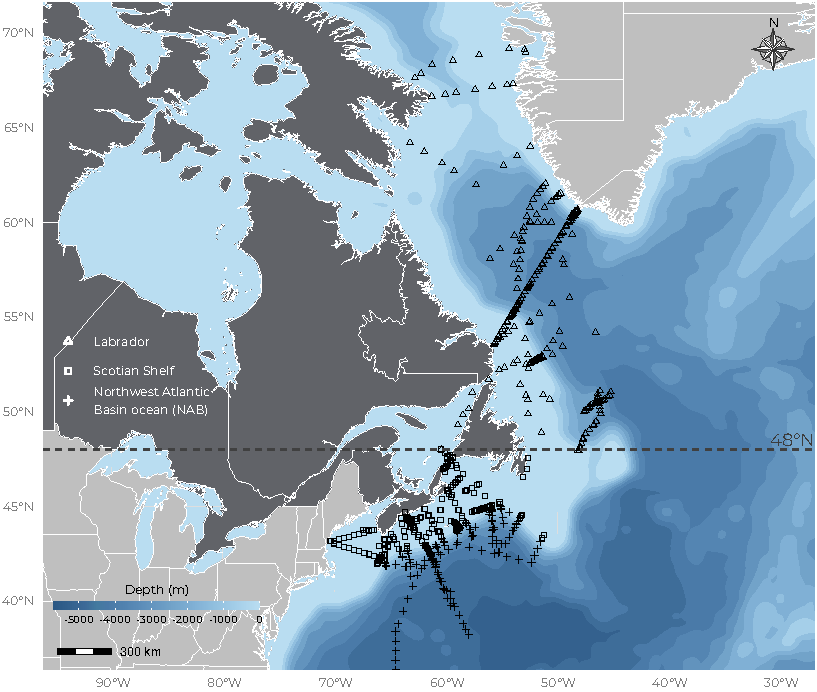
\includegraphics[width=16cm]{fig01.pdf}% This is a *.eps file
\end{center}
\caption{Location of Samplings. The blue backgound indicate the bathymetry (see colorbar in bottom left panel). Dark grey corresponds to Canada and light Grey corresponds to other countries (i.e., United States of America and Denmark}\label{fig:1}
\end{figure}


\begin{figure}[h!]
\begin{center}
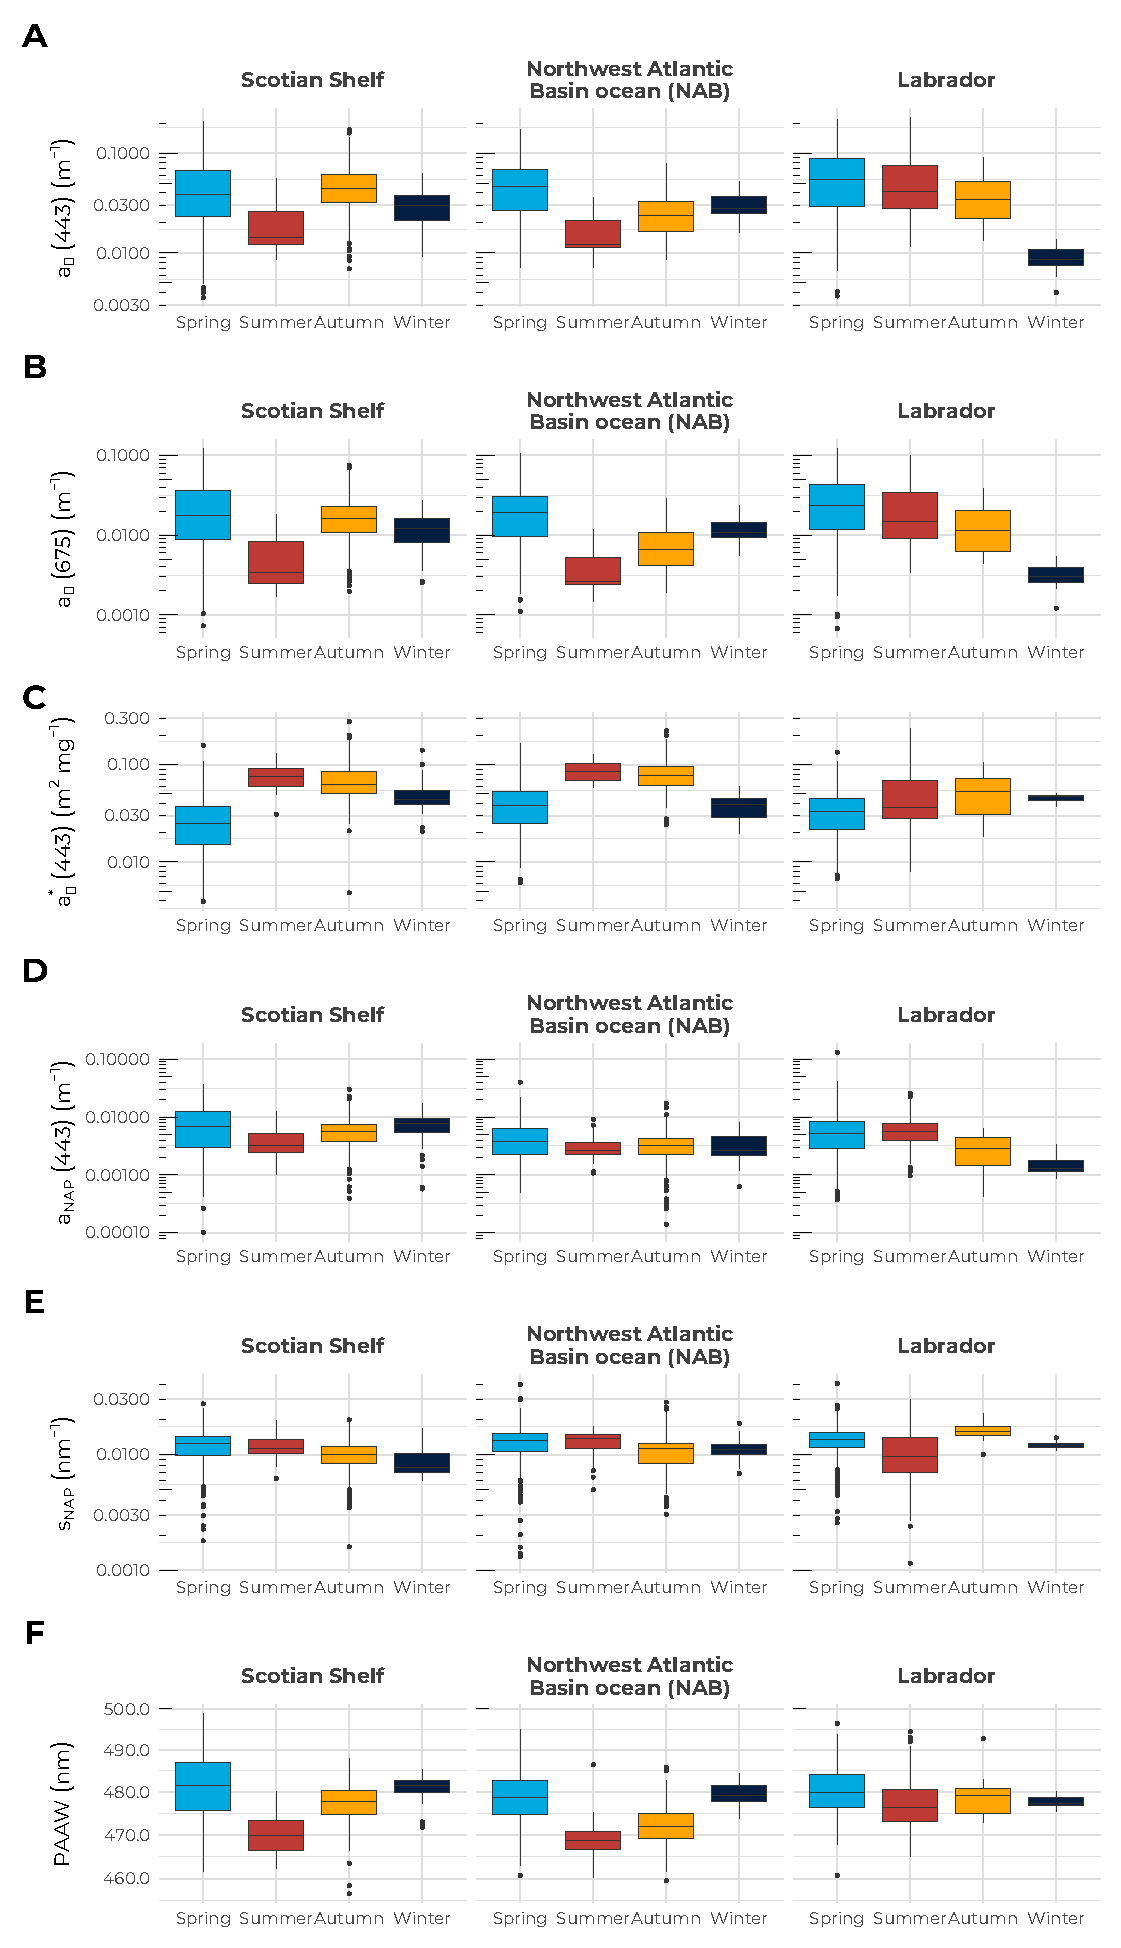
\includegraphics[width=12cm]{fig02.pdf}
\end{center}
\caption{Mean and one standard deviation (i.e., boxplot) of A) $a_\phi(443)$, B)$a_\phi(675)$, C) $a^*_\phi(443)$, D) $a_{NAP}(443)$, E) $S_{NAP}$ and F) $PAAW$ for the Scotian Shelf (left column), Northwest Atlantic Ocean (middle column) and Labrador Sea (right column). In each panel, the blue, red, yellow and black boxes correspond to the spring, summer, autumn and winter respectively. }\label{fig:2}
\end{figure}

\begin{figure}[h!]
\begin{center}
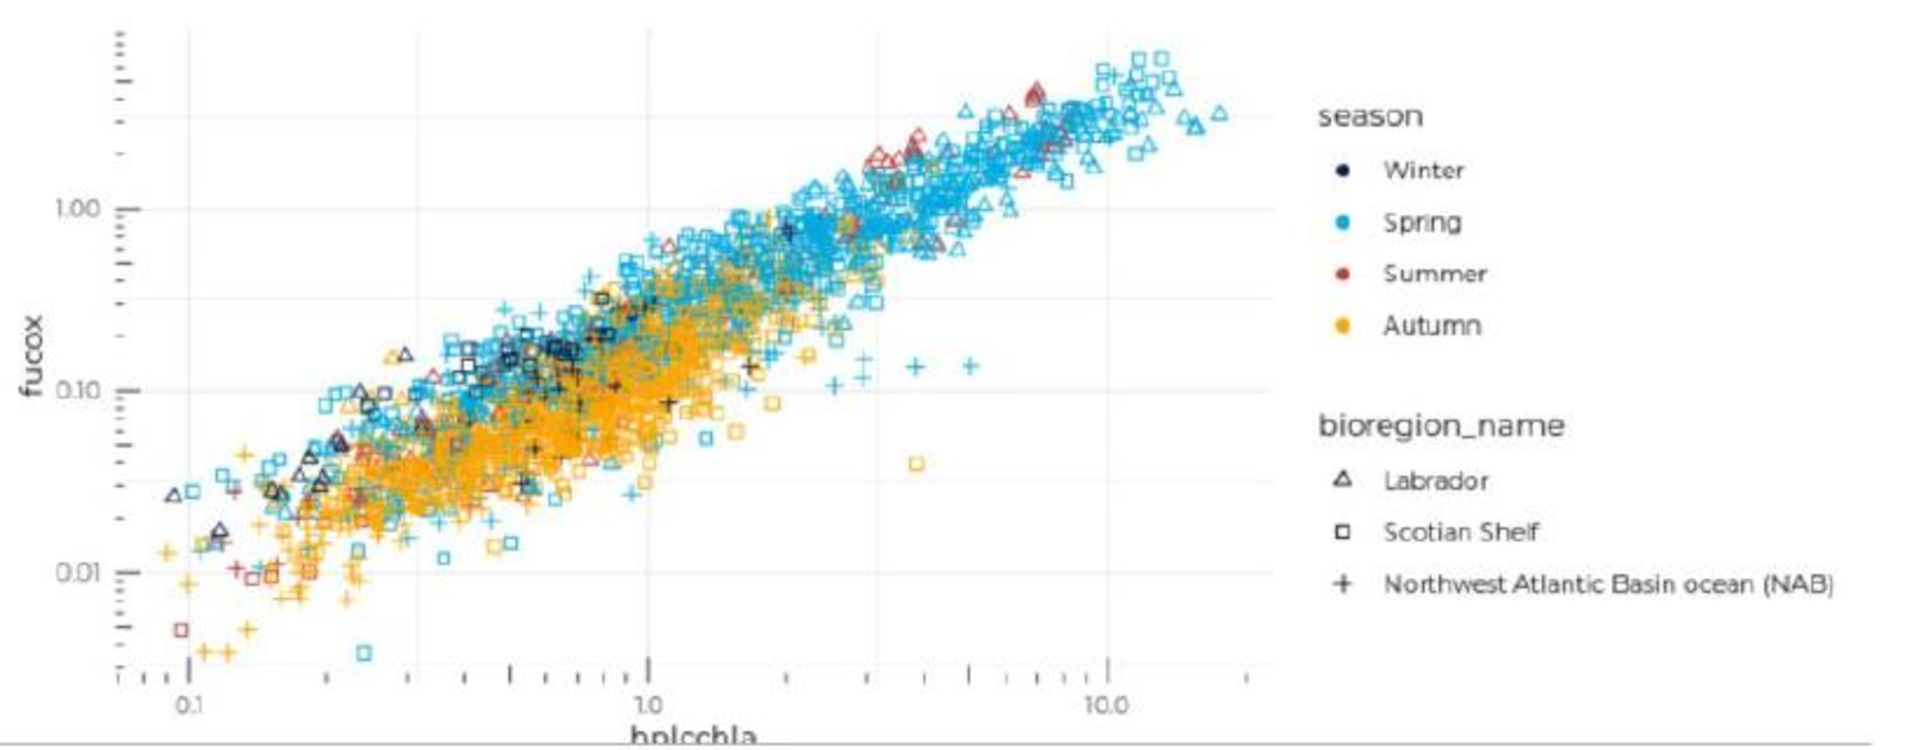
\includegraphics[width=16cm]{fig03.pdf}
\end{center}
\caption{[Fucox] as a functin of [Chl-a]. Symbols are colour coded according to season as in Figure \ref{fig:2}}\label{fig:3}
\end{figure}

\begin{figure}[h!]
\begin{center}
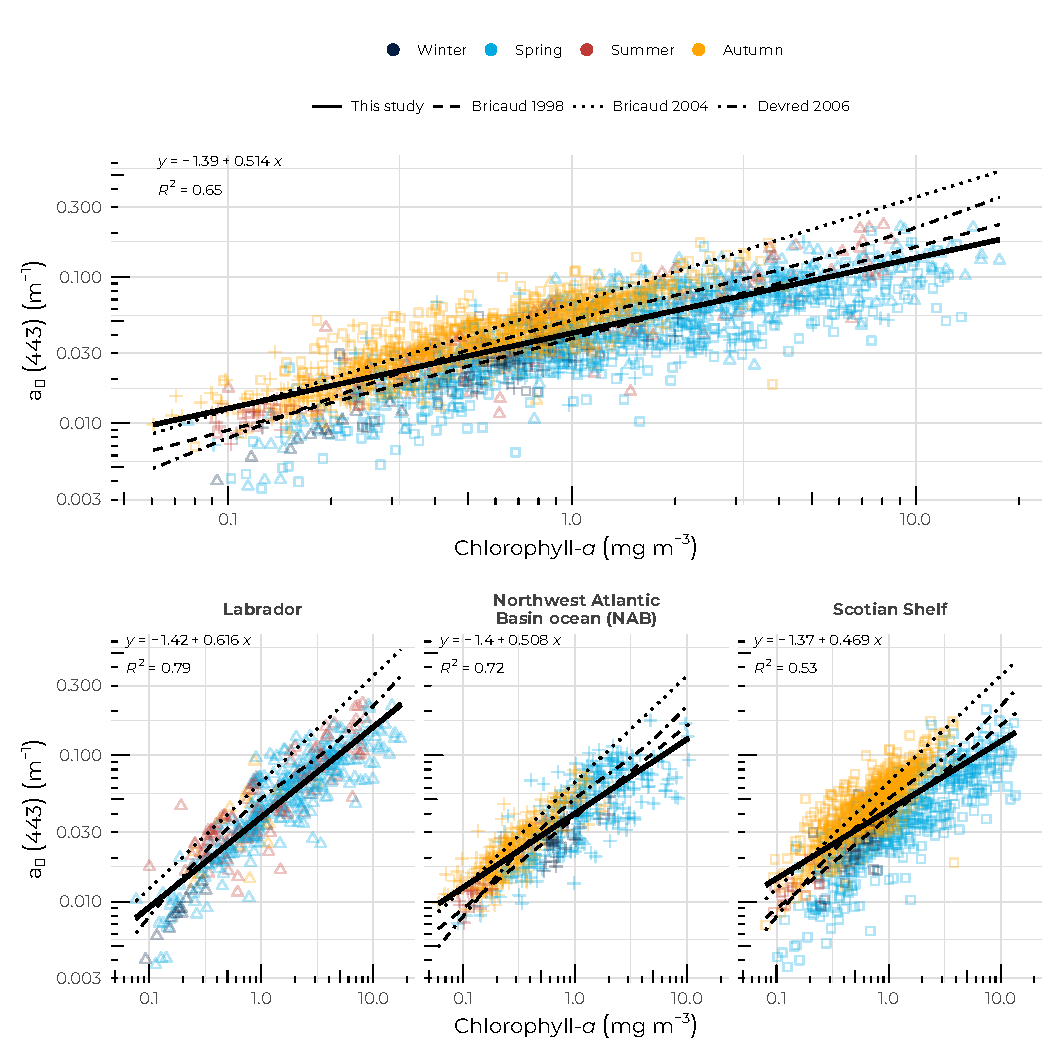
\includegraphics[width=16cm]{fig04.pdf}
\end{center}
\caption{Phytoplankton absorption coefficient at 443\,nm, $a_\phi(443)$, as a function of [Chl-a] for A) the entire dataset, B) the Scotian Shelf, C) the Northwest Atlantic Basin and D) the Labrador Sea. The solid black lines correspond to the power law fit (Equation \ref{eq:3}), the long-dahsed, short-dahsed and dotted-dahsed lines correspond to \cite{bricaud1998}, \cite{bricaud2004} and \cite{devred2006} models respectively. Symbols are colour coded according to season as in Figure \ref{fig:2}}\label{fig:4}
\end{figure}

\begin{figure}[h!]
\begin{center}
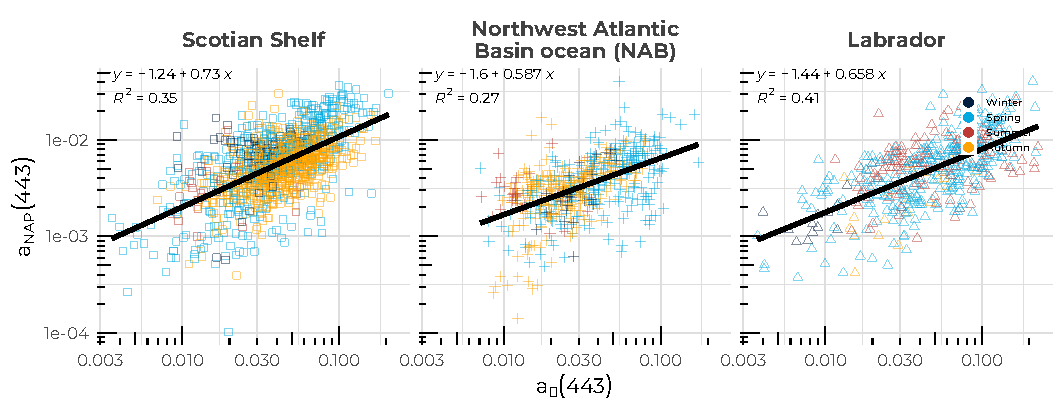
\includegraphics[width=16cm]{fig05.pdf}
\end{center}
\caption{\textcolor{red}{can you group figure 5 and 5b together as in figure \ref{fig:4}}. I dont know what you mean. In the legend you talk about chl and this figure do not show cha. Also, I do not know what is fig 5b, you changed the figure order. Non-algal particulate absorption coefficient at 443\,nm, $a_{NAP}(443)$, as a function of [Chl-a] for A) the entire dataset, B) the Scotian Shelf, C) the Northwest Atlantic Basin and D) the Labrador Sea. The solid black lines correspond to the power law fit (Equation \ref{eq:3}), the long-dahsed, short-dahsed and dotted-dahsed lines correspond to \cite{bricaud1998}, \cite{bricaud2004} and \cite{devred2006} models respectively. Symbols are colour coded according to season as in Figure \ref{fig:2}}\label{fig:5}
\end{figure}

\begin{figure}[h!]
\begin{center}
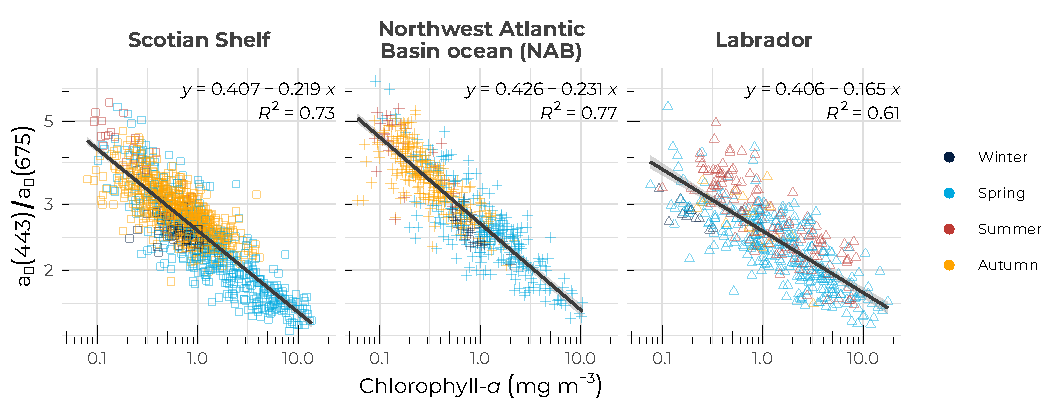
\includegraphics[width=16cm]{fig06.pdf}
\end{center}
\caption{Ratio of $a_\phi(443)$ to $a_\phi(675)$ as a function of [Chl-a] for the Scotian Shelf (left), Northwest Atlantic Basin (middle) and Labrador Sea (right). Symbols are colour coded according to season as in Figure \ref{fig:2}}\label{fig:6}
\end{figure}

\begin{figure}[h!]
\begin{center}
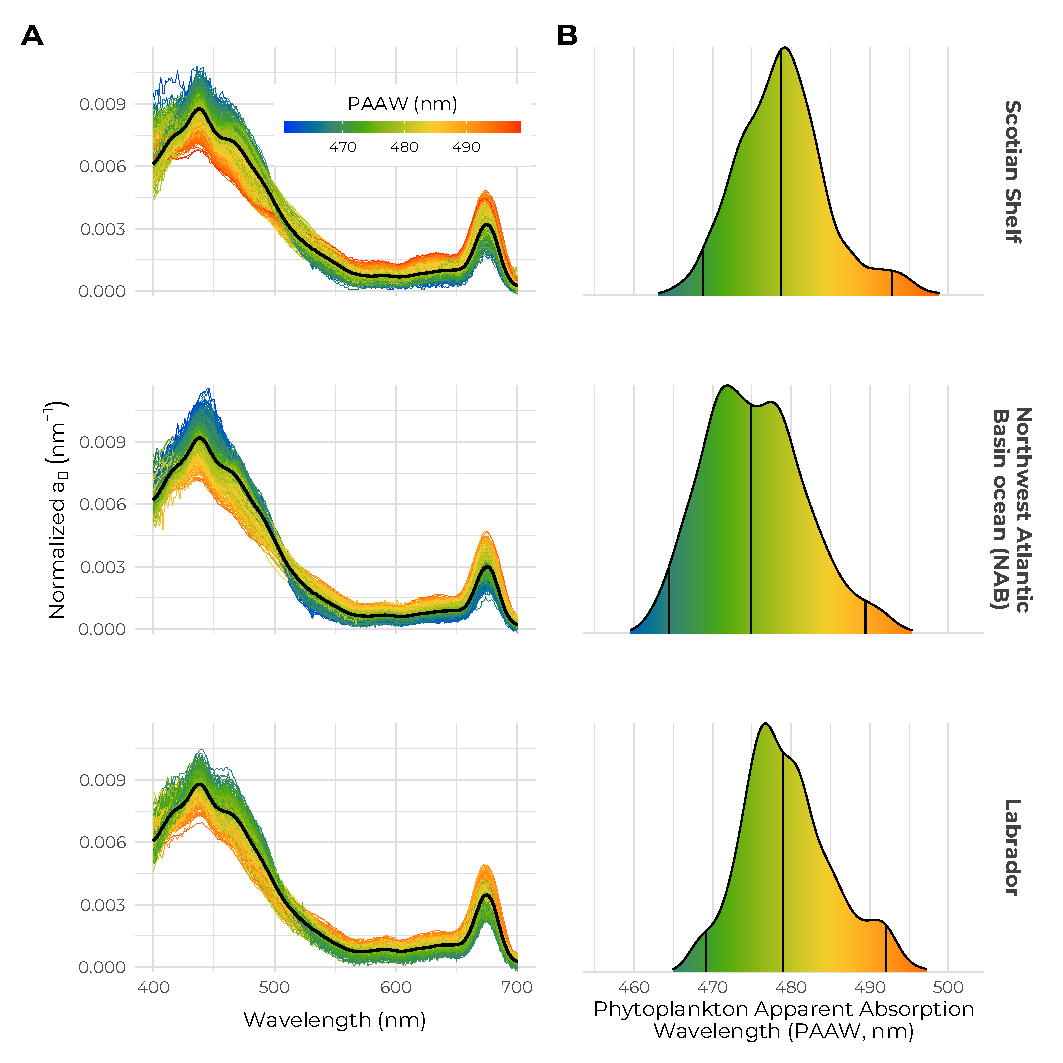
\includegraphics[width=8cm]{fig07.pdf}
\end{center}
\caption{A) Phytoplankton absorption spectra and B) distribution of the $PAAW$ for the Scotian Shelf (top), NAB (middle) and Labrador Sea (bottom), the color bar indicate the $PAAW$ values in all panels.}\label{fig:7}
\end{figure}

\begin{figure}[h!]
\begin{center}
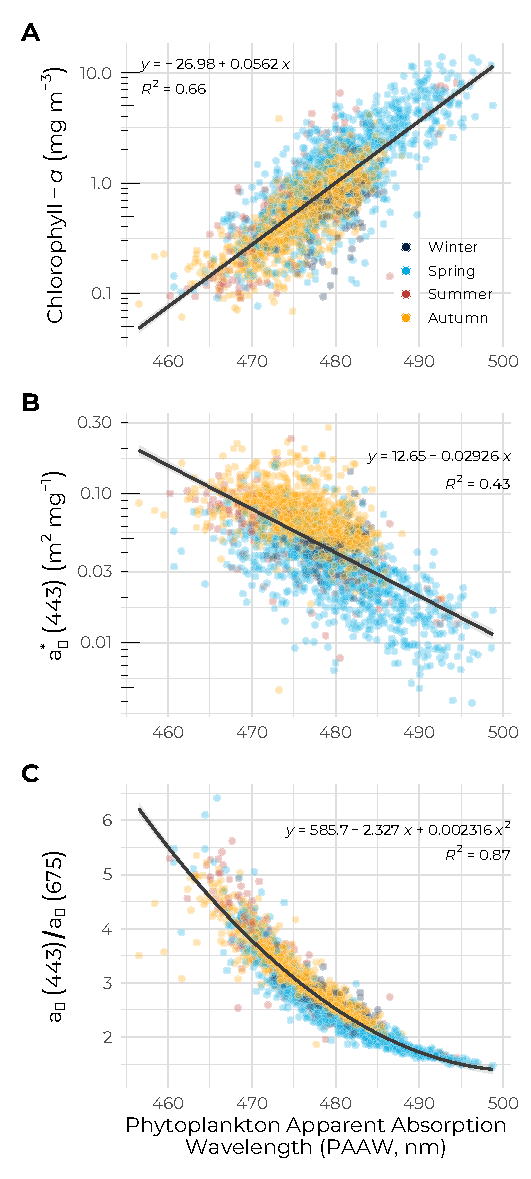
\includegraphics[width=10cm]{fig08.pdf}
\end{center}
\caption{A) [Chl-a], B) $a^*_\phi(443)$ and C) $a_\phi(443):a_\phi(675)$ as a function of $PAAW$ for the entire dataset}\label{fig:8}
\end{figure}

\begin{figure}[h!]
\begin{center}
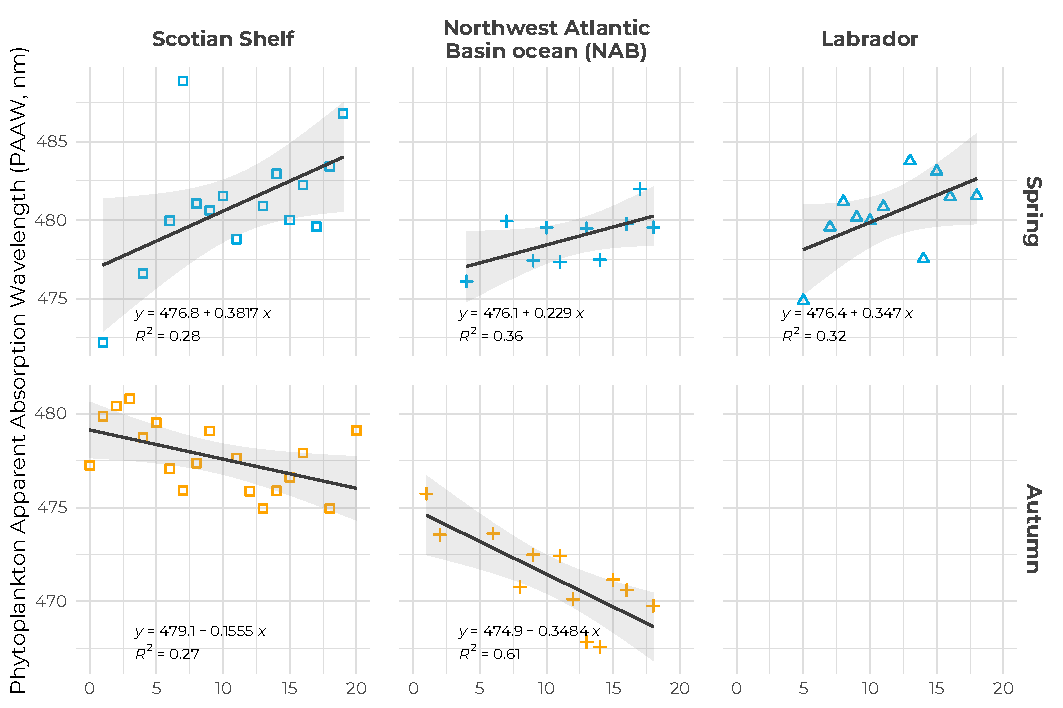
\includegraphics[width=16cm]{fig09.pdf}
\end{center}
\caption{Seasonal trends in $PAAW$ for spring (top panels) and autumn (bottom panels) for the Scotian Shelf (left), NAB (middle) and Labrador Sea (right). The black solid lines correspond to the linear regression of $PAAW$ against time witht the coefficient and $R^2$ indicated in each panel. Symbols are colour coded according to season as in Figure \ref{fig:2}}\label{fig:9}
\end{figure}

\begin{figure}[h!]
\begin{center}
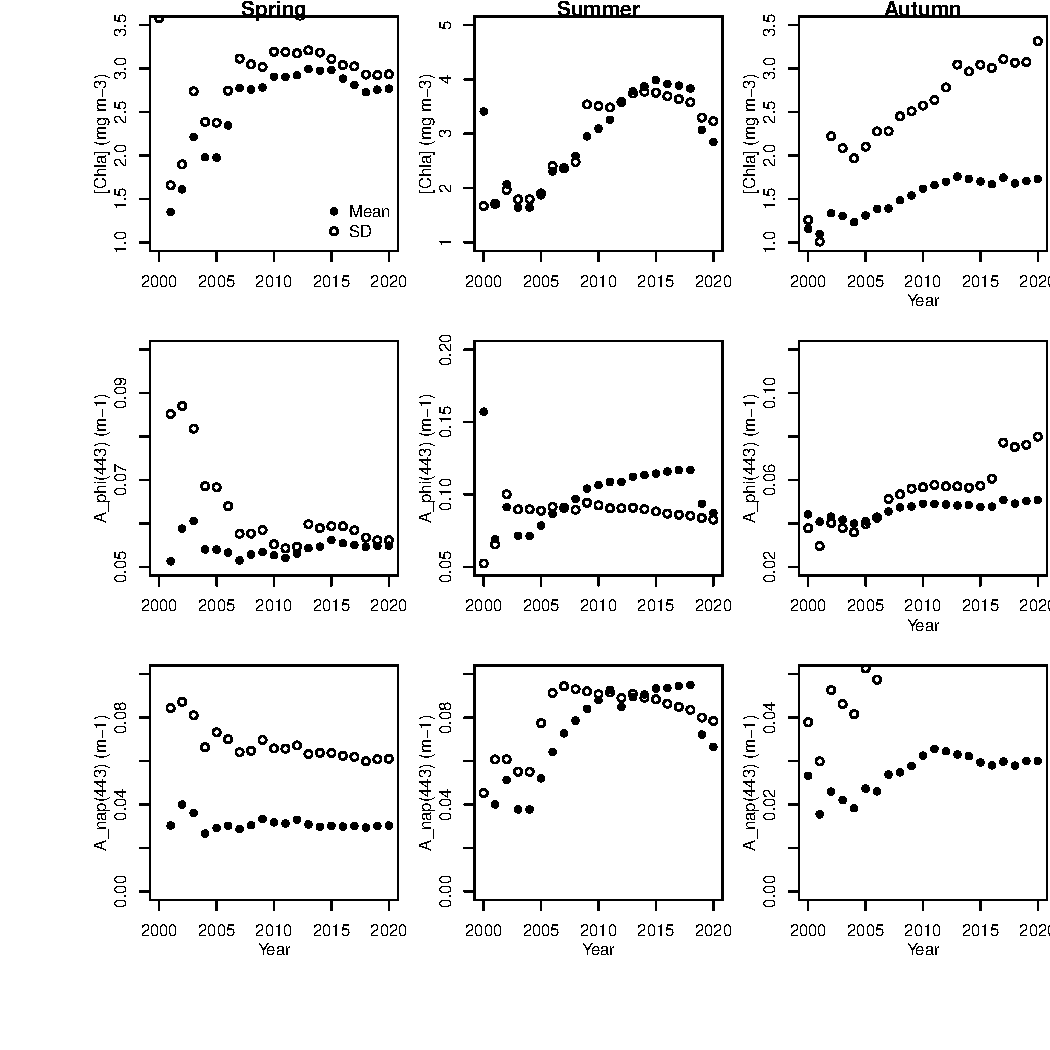
\includegraphics[width=16cm]{fig10.pdf}
\end{center}
\caption{Mean (solid black circles) and standard deviation (open black circle) as a function of time for [Chl-a] (top), $a_\phi(443)$ (middle) and $a_{NAP}(443)$ (bottom) (you should use text mode to write NAP instead of math mode, it does not look good) in spring (left column), summer (middle column) and autumn (right column on the Scotian Shelf}\label{fig:10}
\end{figure}
%%% If you are submitting a figure with subfigures please combine these into one image file with part labels integrated.
%%% If you don't add the figures in the LaTeX files, please upload them when submitting the article.
%%% Frontiers will add the figures at the end of the provisional pdf automatically
%%% The use of LaTeX coding to draw Diagrams/Figures/Structures should be avoided. They should be external callouts including graphics.

\end{document}
